\documentclass[ignorenonframetext,]{beamer}
\setbeamertemplate{caption}[numbered]
\setbeamertemplate{caption label separator}{: }
\setbeamercolor{caption name}{fg=normal text.fg}
\beamertemplatenavigationsymbolsempty
\usepackage{lmodern}
\usepackage{amssymb,amsmath}
\usepackage{ifxetex,ifluatex}
\usepackage{fixltx2e} % provides \textsubscript
\ifnum 0\ifxetex 1\fi\ifluatex 1\fi=0 % if pdftex
\usepackage[T1]{fontenc}
\usepackage[utf8]{inputenc}
\else % if luatex or xelatex
\ifxetex
\usepackage{mathspec}
\else
\usepackage{fontspec}
\fi
\defaultfontfeatures{Ligatures=TeX,Scale=MatchLowercase}
\fi
\usecolortheme{beaver}
% use upquote if available, for straight quotes in verbatim environments
\IfFileExists{upquote.sty}{\usepackage{upquote}}{}
% use microtype if available
\IfFileExists{microtype.sty}{%
\usepackage{microtype}
\UseMicrotypeSet[protrusion]{basicmath} % disable protrusion for tt fonts
}{}
\newif\ifbibliography
\usepackage{color}
\usepackage{fancyvrb}
\newcommand{\VerbBar}{|}
\newcommand{\VERB}{\Verb[commandchars=\\\{\}]}
\DefineVerbatimEnvironment{Highlighting}{Verbatim}{commandchars=\\\{\}}
% Add ',fontsize=\small' for more characters per line
\usepackage{framed}
\definecolor{shadecolor}{RGB}{248,248,248}
\newenvironment{Shaded}{\begin{snugshade}}{\end{snugshade}}
\newcommand{\KeywordTok}[1]{\textcolor[rgb]{0.13,0.29,0.53}{\textbf{{#1}}}}
\newcommand{\DataTypeTok}[1]{\textcolor[rgb]{0.13,0.29,0.53}{{#1}}}
\newcommand{\DecValTok}[1]{\textcolor[rgb]{0.00,0.00,0.81}{{#1}}}
\newcommand{\BaseNTok}[1]{\textcolor[rgb]{0.00,0.00,0.81}{{#1}}}
\newcommand{\FloatTok}[1]{\textcolor[rgb]{0.00,0.00,0.81}{{#1}}}
\newcommand{\ConstantTok}[1]{\textcolor[rgb]{0.00,0.00,0.00}{{#1}}}
\newcommand{\CharTok}[1]{\textcolor[rgb]{0.31,0.60,0.02}{{#1}}}
\newcommand{\SpecialCharTok}[1]{\textcolor[rgb]{0.00,0.00,0.00}{{#1}}}
\newcommand{\StringTok}[1]{\textcolor[rgb]{0.31,0.60,0.02}{{#1}}}
\newcommand{\VerbatimStringTok}[1]{\textcolor[rgb]{0.31,0.60,0.02}{{#1}}}
\newcommand{\SpecialStringTok}[1]{\textcolor[rgb]{0.31,0.60,0.02}{{#1}}}
\newcommand{\ImportTok}[1]{{#1}}
\newcommand{\CommentTok}[1]{\textcolor[rgb]{0.56,0.35,0.01}{\textit{{#1}}}}
\newcommand{\DocumentationTok}[1]{\textcolor[rgb]{0.56,0.35,0.01}{\textbf{\textit{{#1}}}}}
\newcommand{\AnnotationTok}[1]{\textcolor[rgb]{0.56,0.35,0.01}{\textbf{\textit{{#1}}}}}
\newcommand{\CommentVarTok}[1]{\textcolor[rgb]{0.56,0.35,0.01}{\textbf{\textit{{#1}}}}}
\newcommand{\OtherTok}[1]{\textcolor[rgb]{0.56,0.35,0.01}{{#1}}}
\newcommand{\FunctionTok}[1]{\textcolor[rgb]{0.00,0.00,0.00}{{#1}}}
\newcommand{\VariableTok}[1]{\textcolor[rgb]{0.00,0.00,0.00}{{#1}}}
\newcommand{\ControlFlowTok}[1]{\textcolor[rgb]{0.13,0.29,0.53}{\textbf{{#1}}}}
\newcommand{\OperatorTok}[1]{\textcolor[rgb]{0.81,0.36,0.00}{\textbf{{#1}}}}
\newcommand{\BuiltInTok}[1]{{#1}}
\newcommand{\ExtensionTok}[1]{{#1}}
\newcommand{\PreprocessorTok}[1]{\textcolor[rgb]{0.56,0.35,0.01}{\textit{{#1}}}}
\newcommand{\AttributeTok}[1]{\textcolor[rgb]{0.77,0.63,0.00}{{#1}}}
\newcommand{\RegionMarkerTok}[1]{{#1}}
\newcommand{\InformationTok}[1]{\textcolor[rgb]{0.56,0.35,0.01}{\textbf{\textit{{#1}}}}}
\newcommand{\WarningTok}[1]{\textcolor[rgb]{0.56,0.35,0.01}{\textbf{\textit{{#1}}}}}
\newcommand{\AlertTok}[1]{\textcolor[rgb]{0.94,0.16,0.16}{{#1}}}
\newcommand{\ErrorTok}[1]{\textcolor[rgb]{0.64,0.00,0.00}{\textbf{{#1}}}}
\newcommand{\NormalTok}[1]{{#1}}
\usepackage{graphicx,grffile}
\makeatletter
\def\maxwidth{\ifdim\Gin@nat@width>\linewidth\linewidth\else\Gin@nat@width\fi}
\def\maxheight{\ifdim\Gin@nat@height>\textheight0.8\textheight\else\Gin@nat@height\fi}
\makeatother
% Scale images if necessary, so that they will not overflow the page
% margins by default, and it is still possible to overwrite the defaults
% using explicit options in \includegraphics[width, height, ...]{}
\setkeys{Gin}{width=\maxwidth,height=\maxheight,keepaspectratio}

% Prevent slide breaks in the middle of a paragraph:
\widowpenalties 1 10000
\raggedbottom

\AtBeginPart{
\let\insertpartnumber\relax
\let\partname\relax
\frame{\partpage}
}
\AtBeginSection{
\ifbibliography
\else
\let\insertsectionnumber\relax
\let\sectionname\relax
\frame{\sectionpage}
\fi
}
\AtBeginSubsection{
\let\insertsubsectionnumber\relax
\let\subsectionname\relax
\frame{\subsectionpage}
}

\setlength{\parindent}{0pt}
\setlength{\parskip}{6pt plus 2pt minus 1pt}
\setlength{\emergencystretch}{3em}  % prevent overfull lines
\providecommand{\tightlist}{%
\setlength{\itemsep}{0pt}\setlength{\parskip}{0pt}}
\setcounter{secnumdepth}{0}
%%% Работа с русским языком
\usepackage[russian,english]{babel}   %% загружает пакет многоязыковой вёрстки
\usepackage{fontspec}      %% подготавливает загрузку шрифтов Open Type, True Type и др.
\defaultfontfeatures{Ligatures={TeX},Renderer=Basic,Scale=0.75}  %% свойства шрифтов по умолчанию
\setmainfont[Ligatures={TeX,Historic}]{Times New Roman} %% задаёт основной шрифт документа
\setsansfont[Ligatures={TeX,Historic}]{Verdana} %% задаёт шрифт без засечек
\setmonofont[Scale=0.7]{DejaVu Sans Mono}

\linespread{0.75}

\definecolor{links}{HTML}{2A1B81}
\hypersetup{colorlinks=true,linkcolor=,urlcolor=links,pdfview=FitH,pdfpagelayout=SinglePage, unicode=true,breaklinks=true}

% links format
\usepackage{hyperref}

% decrease text margins
\setbeamersize{text margin left = 8pt, text margin right = 16pt}

\newcommand{\columnsbegin}{\begin{columns}}
\newcommand{\columnsend}{\end{columns}}
\newcommand{\blockbegin}{\begin{block}}
\newcommand{\blockend}{\end{block}}

\usepackage{graphics}

% % subfigures
% \usepackage{subcaption}
% \usepackage{wrapfig}

%\addto{\captionsrussian}{\renewcommand*{\figurename}{рис.}}

% Tables
% Define new column types to adjust sizes in tabular environment
% For example, \begin{tabular}{ L{2.3cm} C{2cm} C{1.5cm} C{2.5cm} C{4cm}}
\usepackage{array}
\renewcommand{\arraystretch}{2}
\newcolumntype{L}[1]{>{\raggedright\let\newline\\\arraybackslash\hspace{0pt}}m{#1}}
\newcolumntype{C}[1]{>{\centering\let\newline\\\arraybackslash\hspace{0pt}}m{#1}}
\newcolumntype{R}[1]{>{\raggedleft\let\newline\\\arraybackslash\hspace{0pt}}m{#1}}

\logo{
\includegraphics[height=0.3cm]{assets/Linmod_logo.png}}

\title{Регрессионный анализ для бинарных данных}
\subtitle{Линейные модели\ldots{}}
\author{Вадим Хайтов, Марина Варфоломеева}
\date{}

\begin{document}
\frame{\titlepage}

\begin{frame}{Мы рассмотрим}

\begin{itemize}
\tightlist
\item
  Регрессионный анализ для бинарных зависимых переменных
\end{itemize}

\begin{block}{Вы сможете}

\begin{itemize}
\tightlist
\item
  Построить логистическую регрессионную модель, подобранную методом
  максимального правдоподобия
\item
  Дать трактовку параметрам логистической регрессионной модели
\item
  Провести анализ девиансы, основанный на логистической регрессии
\end{itemize}

\end{block}

\end{frame}

\begin{frame}{Бинарные данные - очень распространенный тип зависимых
переменных}

\begin{itemize}
\tightlist
\item
  Вид есть - вида нет
\item
  Кто-то в результате эксперимента выжил или умер
\item
  Пойманное животное заражено паразитами или здорово
\item
  Команда выиграла или проиграла
\end{itemize}

и т.д.

\end{frame}

\begin{frame}[fragile]{На каком острове лучше искать ящериц?}

\columnsbegin

\column{0.5 \textwidth}


\includegraphics[width=\linewidth] {images/esher.jpg}

\column {0.5 \textwidth}

\begin{Shaded}
\begin{Highlighting}[]
\NormalTok{liz <-}\StringTok{ }\KeywordTok{read.csv}\NormalTok{(}\StringTok{"data/polis.csv"}\NormalTok{)}
\KeywordTok{head}\NormalTok{(liz)}
\end{Highlighting}
\end{Shaded}

\begin{verbatim}
#     X.ISLAND PARATIO UTA PA PREDICT
# 1       Bota   15.41   P  1   0.555
# 2     Cabeza    5.63   P  1   0.915
# 3    Cerraja   25.92   P  1   0.111
# 4 Coronadito   15.17   A  0   0.568
# 5     Flecha   13.04   P  1   0.678
# 6   Gemelose   18.85   A  0   0.370
\end{verbatim}

\columnsend

\vskip0pt plus 1filll
\tiny{Пример взят из книги Quinn \& Keugh (2002), Оригинальная работа Polis et al. (1998)}

\end{frame}

\begin{frame}[fragile]{Зависит ли встречаемость ящериц от размера
острова?}

\columnsbegin
\column {0.5 \textwidth}

\begin{small}

Обычную линейную регрессию подобрать можно,

Зависимая переменная: \\
PA - (есть ящерицы "1" - нет ящериц "0")

Предиктор: \\
PARATIO (отношение периметра к площади)


\end{small}

\begin{Shaded}
\begin{Highlighting}[]
\NormalTok{fit <-}\StringTok{ }\KeywordTok{lm}\NormalTok{(PA ~}\StringTok{ }\NormalTok{PARATIO, }\DataTypeTok{data =} \NormalTok{liz)}
\KeywordTok{summary}\NormalTok{(fit)}
\end{Highlighting}
\end{Shaded}

\column {0.5 \textwidth}

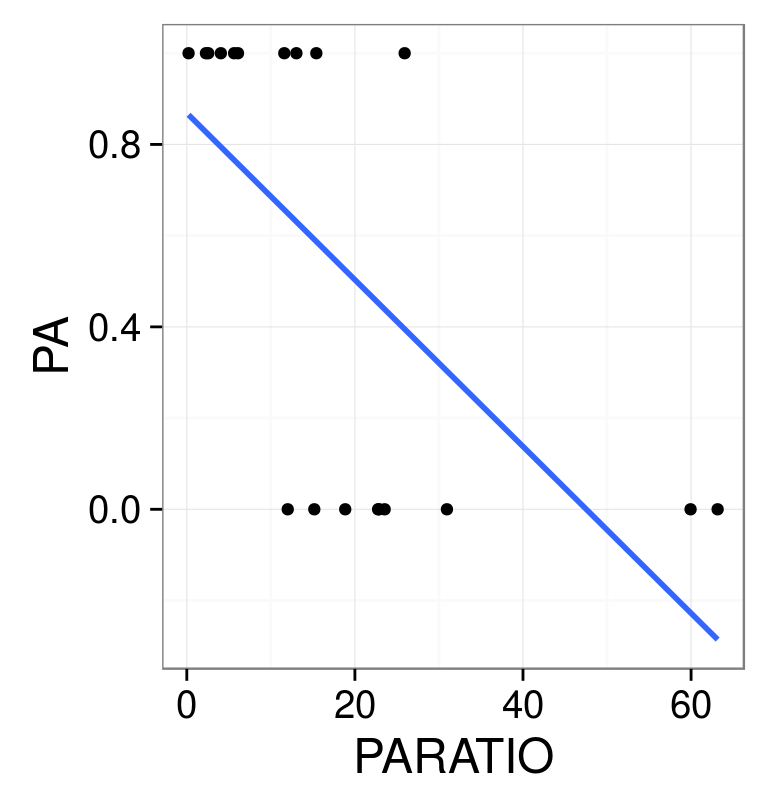
\includegraphics{11_GLM_binary2_files/figure-beamer/unnamed-chunk-3-1.pdf}

\textbf {но она категорически не годится}

\columnsend

\end{frame}

\begin{frame}{Эти данные лучше описывает логистическая кривая}

\columnsbegin

\column {0.5 \textwidth}
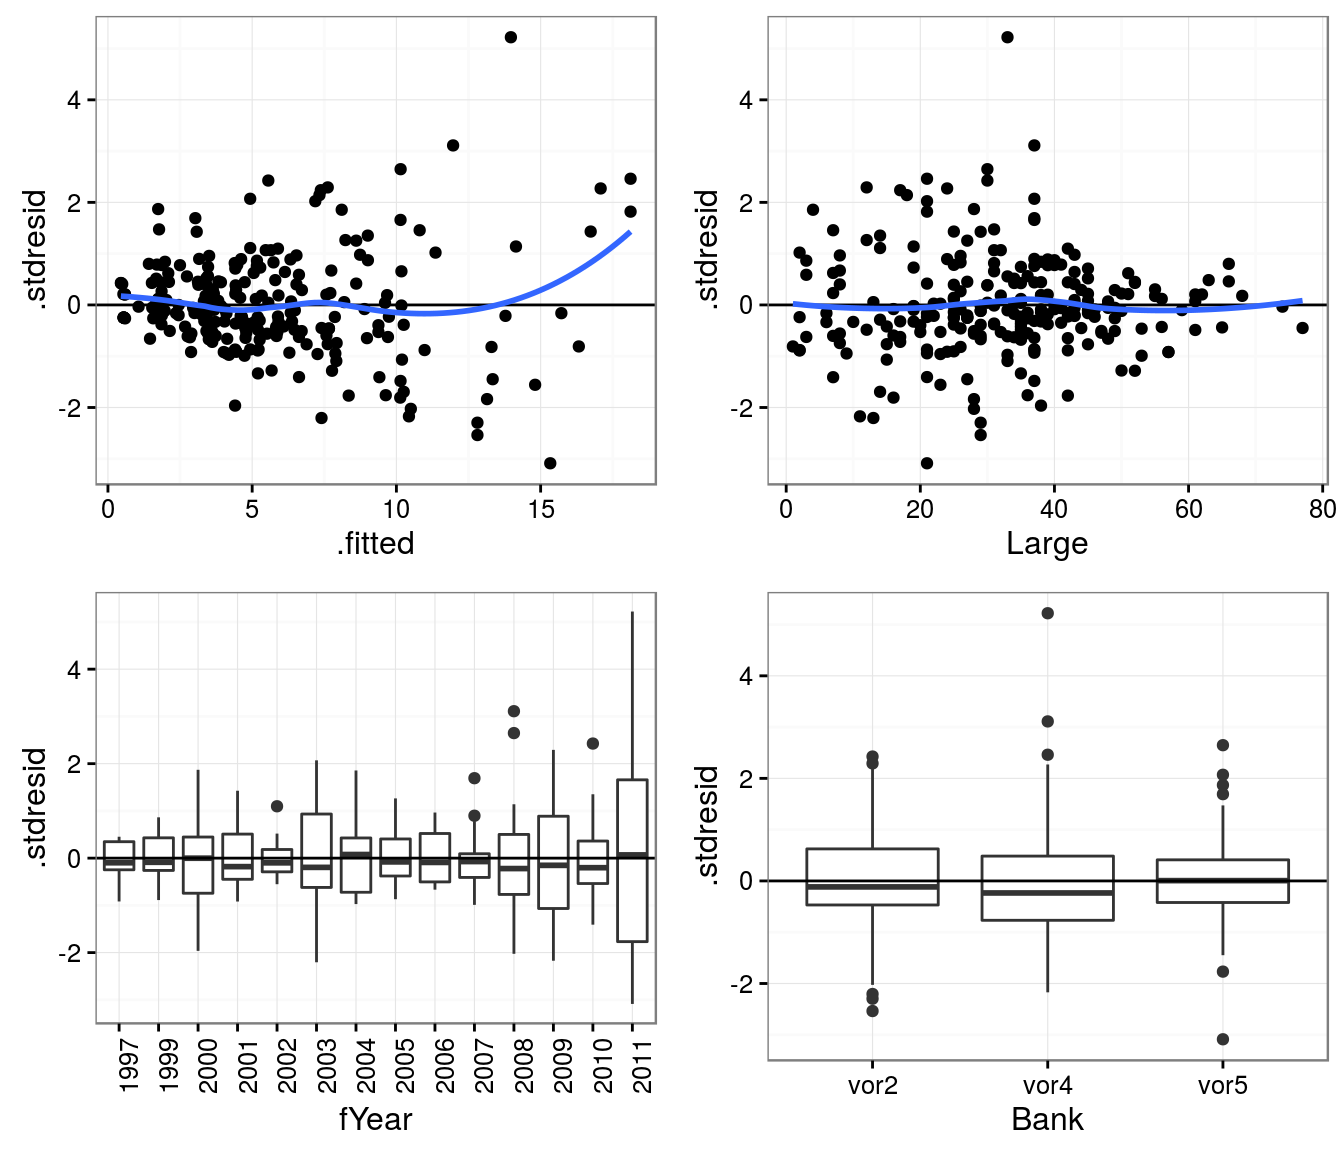
\includegraphics{11_GLM_binary2_files/figure-beamer/unnamed-chunk-4-1.pdf}

\column {0.5 \textwidth} Логистическая кривая описывается такой формулой

\[ \pi(x) = \frac{e^{\beta_0+\beta_1x}}{1+e^{\beta_0+\beta_1x}} \]

\columnsend

\end{frame}

\begin{frame}{Зависимую величину можно преобразовать в более удобную для
моделирования форму}

\begin{enumerate}[<+->]
\def\labelenumi{\arabic{enumi}.}
\tightlist
\item
  Дискретный результат: 1 или 0
\item
  Дискретные данные можно преобразовать в форму оценки вероятности
  события: \(\pi = \frac{N_i}{N_{total}}\), непрерывная аеличина,
  варьирующая от 0 до 1
\item
  Вероятность события можно выразить в форме шансов (odds):
  \(odds=\frac{\pi}{1-\pi}\) варьируют от 0 до \(+\infty\). \emph{NB:
  Если шансы \textgreater{} 1, то вероятность события, что \(y_i=1\)
  выше, чем вероятность события \(y_i = 0\). Если шансы \textless{} 1,
  то наоборот}. В обыденной речи мы часто использем фразы, наподобие
  такой ``\emph{шансы на победу 1 к 3}''
\item
  Шансы преобразуются в \emph{Логиты} (logit):
  \(ln(odds)=\ln(\frac{\pi}{1-\pi})\) варьируют от \(-\infty\) до
  \(+\infty\). Логиты гораздо удобнее для построения моделей.
\end{enumerate}

\end{frame}

\begin{frame}{Что станет с логистической моделью после
логит-преобразования?}

\begin{block}{Немного алгебры}

Обозначим для краткости \(\beta_0 + \beta_1x \equiv z\)

Тогда

\begin{small}
$$ g(x)=\ln(\frac{\pi(x)}{1-\pi(x)})= \ln(\frac{\frac{e^z}{1+e^z}}{1-\frac{e^z}{1+e^z}}) $$
\pause
$$ g(x)=\ln(\frac{e^z}{1+e^z}) - \ln({1-\frac{e^z}{1+e^z}}) $$
\pause
$$ g(x)=\ln(\frac{e^z}{1+e^z}) - \ln({\frac{1+e^z - e^z}{1+e^z}}) = \ln(\frac{e^z}{1+e^z}) - \ln({\frac{1}{1+e^z}})  $$
\pause
$$ g(x)=\ln(e^z) - \ln(1+e^z) - (\ln(1) -\ln(1+e^z))  $$
\pause
$$ g(x)=\ln(e^z) - \ln(1+e^z) - 0 +\ln(1+e^z) = \ln(e^z) = z $$
\end{small}

\end{block}

\end{frame}

\begin{frame}{Логистическая модель после логит-преобразования становится
линейной}

\[ g(x)=\ln(\frac{\pi(x)}{1-\pi(x)})=\beta_0 + \beta_1x\]

Остается только подобрать параметры этой линейной модели: \(\beta_0\)
(интерсепт) и \(\beta_1\) (угловой коэффициент)

\end{frame}

\begin{frame}{Метод максимального правдоподобия}

\begin{block}{Вспомним}

Если остатки не подчиняется нормальному распределению, то метод
наименьших квадратов не работает.\\
В этом случае применяют \emph{Метод максимального правдоподбия}

В результате итеративных процедур происходит подбор таких значений
коэффициентов, при которых правдоподобие - вероятность получения
имеющегося у нас набора данных - оказывается максимальным, при условии
справедливости данной модели.

\[ Lik(x_1, ..., x_n) = \Pi^n _{i = 1}f(x_i; \theta)\]

где \(f(x; \theta)\) - функция плотности вероятности с параметрами
\(\theta\)

\end{block}

\end{frame}

\begin{frame}{Правдоподобие для биномиального распределения}

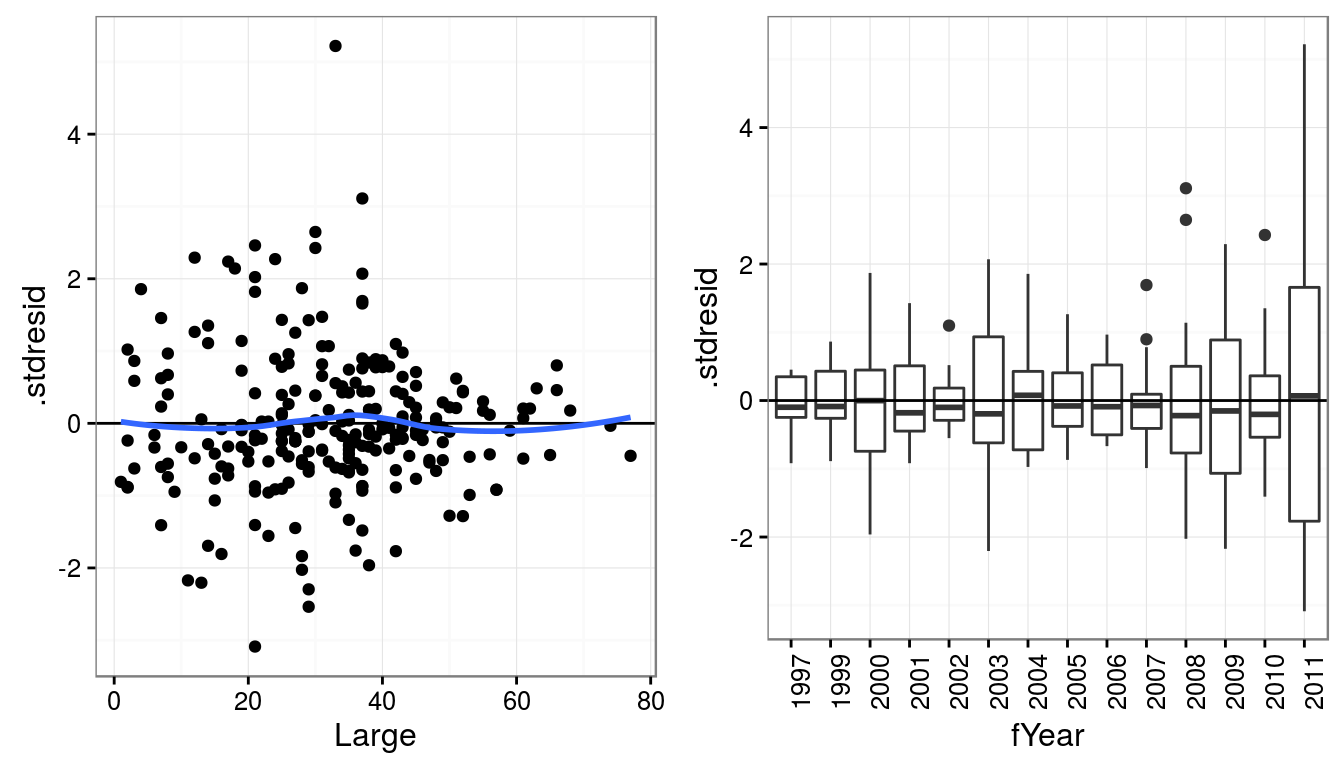
\includegraphics{11_GLM_binary2_files/figure-beamer/unnamed-chunk-5-1.pdf}

\end{frame}

\begin{frame}{Функция правдоподобия для биномиального распределения}

Для случая биномиального распределения \(x \in Bin(n, \pi)\) функция
правдоподобия имеет следующий вид:

\[Lik(\pi|x) = \frac{n!}{(n-x)!x!}\pi^x(1-\pi)^{n-x}\]

отбросив константу, получаем:

\[Lik(\pi|x) \propto \pi^x(1-\pi)^{n-x}\]

\begin{block}{Логарифм правдоподобия}

Удобнее работать с логарифмом функции правдоподобия - \(logLik\) - его
легче максимизировать. В случае биномиального распределения он выглядит
так:

\[logLik(\pi|x) = x log(\pi) + (n-x)log(1-\pi)\]

\end{block}

\end{frame}

\begin{frame}[fragile]{Подберем модель}

\begin{Shaded}
\begin{Highlighting}[]
\NormalTok{liz_model <-}\StringTok{ }\KeywordTok{glm}\NormalTok{(PA ~}\StringTok{ }\NormalTok{PARATIO , }\DataTypeTok{family=}\StringTok{"binomial"}\NormalTok{, }\DataTypeTok{data =} \NormalTok{liz)}
\KeywordTok{summary}\NormalTok{(liz_model)}
\end{Highlighting}
\end{Shaded}

\begin{verbatim}
# 
# Call:
# glm(formula = PA ~ PARATIO, family = "binomial", data = liz)
# 
# Deviance Residuals: 
#    Min      1Q  Median      3Q     Max  
# -1.607  -0.638   0.237   0.433   2.099  
# 
# Coefficients:
#             Estimate Std. Error z value Pr(>|z|)  
# (Intercept)    3.606      1.695    2.13    0.033 *
# PARATIO       -0.220      0.101   -2.18    0.029 *
# ---
# Signif. codes:  0 '***' 0.001 '**' 0.01 '*' 0.05 '.' 0.1 ' ' 1
# 
# (Dispersion parameter for binomial family taken to be 1)
# 
#     Null deviance: 26.287  on 18  degrees of freedom
# Residual deviance: 14.221  on 17  degrees of freedom
# AIC: 18.22
# 
# Number of Fisher Scoring iterations: 6
\end{verbatim}

\end{frame}

\begin{frame}[fragile]{\texttt{summary()} для модели, подобранной
методом максимального правдоподобия}

\begin{verbatim}
# 
# Call:
# glm(formula = PA ~ PARATIO, family = "binomial", data = liz)
# 
# Deviance Residuals: 
#    Min      1Q  Median      3Q     Max  
# -1.607  -0.638   0.237   0.433   2.099  
# 
# Coefficients:
#             Estimate Std. Error z value Pr(>|z|)  
# (Intercept)    3.606      1.695    2.13    0.033 *
# PARATIO       -0.220      0.101   -2.18    0.029 *
# ---
# Signif. codes:  0 '***' 0.001 '**' 0.01 '*' 0.05 '.' 0.1 ' ' 1
# 
# (Dispersion parameter for binomial family taken to be 1)
# 
#     Null deviance: 26.287  on 18  degrees of freedom
# Residual deviance: 14.221  on 17  degrees of freedom
# AIC: 18.22
# 
# Number of Fisher Scoring iterations: 6
\end{verbatim}

Есть уже знакомые термины: \texttt{Estimate}, \texttt{Std.\ Error},
\texttt{AIC}\\
Появились новые термины: \texttt{z\ value},
\texttt{Pr(\textgreater{}\textbar{}z\textbar{})},
\texttt{Null\ deviance}, \texttt{Residual\ deviance}

\end{frame}

\begin{frame}{``z value''" и ``Pr(\textgreater{}z)''}

z - это величина критерия Вальда (\emph{Wald statistic}) - аналог
t-критерия

Используется для проверки \(H_0: \beta_1=0\)

\[z=\frac{\beta_1}{SE_{\beta_1}}\]

Сравнивают со стандартным нормальным распределением (z-распределение)

Дает надежные оценки p-value при больших выборках

\end{frame}

\begin{frame}{Null deviance и Residual deviance}

Имеющиеся данные позволяют ``вписать'' три типа моделей

\textbf{``Насыщенная'' модель} - модель, подразумевающая, что каждая из
n точек имеет свой собственный параметр, следовательно надо подобрать n
параметров. Вероятность существования данных для такой модели равна 1.
\[logLik_{satur}=0\]
\[df_{saturated} = n - npar_{saturated}  = n - n = 0\]

\textbf{``Нулевая'' модель} - модель, подразумевающая, что для описания
всех точек надо подобрать только 1 параметр. \(g(x) = \beta_0\).
\[logLik_{nul} \ne 0\] \[df_{null} = n - npar_{null} = n - 1\]

\textbf{``Предложенная'' модель} - модель, подобранная в нашем анализе
\(g(x) = \beta_0 + \beta_1x\) \[logLik_{prop} \ne 0\]
\[df_{proposed} = n - npar_{proposed}\]

\end{frame}

\begin{frame}[fragile]{Null deviance и Residual deviance}

\textbf{Девианса} - это оценка отклонения логарифма максимального
правдоподобия одной модели от логарифма максимального правдоподобия
другой модели

\textbf{Остаточная девианса}:\\
\(Dev_{resid} = 2(logLik_{satur} - logLik_{prop})=-2logLik_{prop}\)

\textbf{Нулевая девианса}:\\
\(Dev_{nul} = 2(logLik_{satur} - logLik_{nul})=-2logLik_{nul}\)

Проверим, совпадут ли со значениями из \texttt{summary()}

\begin{Shaded}
\begin{Highlighting}[]
\NormalTok{(Dev_resid <-}\StringTok{ }\NormalTok{-}\DecValTok{2}\NormalTok{*}\KeywordTok{as.numeric}\NormalTok{(}\KeywordTok{logLik}\NormalTok{(liz_model))) }\CommentTok{#Остаточная девианса}
\end{Highlighting}
\end{Shaded}

\begin{verbatim}
# [1] 14.2
\end{verbatim}

\begin{Shaded}
\begin{Highlighting}[]
\NormalTok{(Dev_nul <-}\StringTok{ }\NormalTok{-}\DecValTok{2}\NormalTok{*}\KeywordTok{as.numeric}\NormalTok{(}\KeywordTok{logLik}\NormalTok{(}\KeywordTok{update}\NormalTok{(liz_model, ~-PARATIO)))) }\CommentTok{#Нулевая девианса}
\end{Highlighting}
\end{Shaded}

\begin{verbatim}
# [1] 26.3
\end{verbatim}

\end{frame}

\begin{frame}[fragile]{Анализ девиансы}

\textbf{По соотношению нулевой девиансы и остаточной девиансы можно
понять насколько статистически значима модель}

В основе анализа девиансы лежит критерий \(G^2\)

\[ G^2 = -2(logLik_{nul} - logLik_{prop})\]

\begin{Shaded}
\begin{Highlighting}[]
\NormalTok{(G2 <-}\StringTok{ }\NormalTok{Dev_nul -}\StringTok{ }\NormalTok{Dev_resid)}
\end{Highlighting}
\end{Shaded}

\begin{verbatim}
# [1] 12.1
\end{verbatim}

Вспомним тест отношения правдоподобий:
\[ LRT = 2ln(Lik_1/Lik_2) = 2(logLik_1 - logLlik_2)\]

\begin{quote}
Тест \(G^2\) - это частный случай теста отношения правдоподобий
(Likelihood Ratio Test)
\end{quote}

\end{frame}

\begin{frame}{Свойства критерия \(G^2\)}

\begin{itemize}[<+->]
\tightlist
\item
  \(G^2\) - это девианса полной (предложенной) и редуцированной модели
  (нулевой)\\
\item
  \(G^2\) - аналог частного F критерия в обычном регрессионном анализе\\
\item
  \(G^2\) - подчиняется \(\chi^2\) распределению (с параметом df = 1)
  если нулевая модель и предложенная модель не отличаются друг от друга.
\item
  \(G^2\) можно использовать для проверки гипотезы о равенстве нулевой и
  остаточной девианс.
\end{itemize}

\end{frame}

\begin{frame}[fragile]{Задание}

\begin{enumerate}
\def\labelenumi{\arabic{enumi}.}
\tightlist
\item
  Вычислите вручную значение критерия \(G^2\) для модели, описывающей
  встречаемость ящериц (\texttt{liz\_model})
\item
  Оцените уровень значимости для него
\end{enumerate}

\[ G^2 = -2(logLik_{nul} - logLik_{prop})\]

\end{frame}

\begin{frame}[fragile]{Решение}

\begin{Shaded}
\begin{Highlighting}[]
\CommentTok{#Остаточная девианса}
\NormalTok{Dev_resid <-}\StringTok{ }\NormalTok{-}\DecValTok{2}\NormalTok{*}\KeywordTok{as.numeric}\NormalTok{(}\KeywordTok{logLik}\NormalTok{(liz_model)) }

\CommentTok{#Нулевая девианса}
\NormalTok{Dev_nul <-}\StringTok{ }\NormalTok{-}\DecValTok{2}\NormalTok{*}\KeywordTok{as.numeric}\NormalTok{(}\KeywordTok{logLik}\NormalTok{(}\KeywordTok{update}\NormalTok{(liz_model, ~-PARATIO)))}

\CommentTok{# Значение критерия }
\NormalTok{(G2 <-}\StringTok{ }\NormalTok{Dev_nul -}\StringTok{ }\NormalTok{Dev_resid)}
\end{Highlighting}
\end{Shaded}

\begin{verbatim}
# [1] 12.1
\end{verbatim}

\begin{Shaded}
\begin{Highlighting}[]
\NormalTok{(p_value <-}\StringTok{ }\DecValTok{1} \NormalTok{-}\StringTok{ }\KeywordTok{pchisq}\NormalTok{(G2, }\DataTypeTok{df =} \DecValTok{1}\NormalTok{))}
\end{Highlighting}
\end{Shaded}

\begin{verbatim}
# [1] 0.000513
\end{verbatim}

\end{frame}

\begin{frame}[fragile]{Решение с помощью функции \texttt{anova()}}

\begin{Shaded}
\begin{Highlighting}[]
\KeywordTok{anova}\NormalTok{(liz_model, }\DataTypeTok{test=}\StringTok{"Chi"}\NormalTok{)}
\end{Highlighting}
\end{Shaded}

\begin{verbatim}
# Analysis of Deviance Table
# 
# Model: binomial, link: logit
# 
# Response: PA
# 
# Terms added sequentially (first to last)
# 
# 
#         Df Deviance Resid. Df Resid. Dev Pr(>Chi)    
# NULL                       18       26.3             
# PARATIO  1     12.1        17       14.2  0.00051 ***
# ---
# Signif. codes:  0 '***' 0.001 '**' 0.01 '*' 0.05 '.' 0.1 ' ' 1
\end{verbatim}

\end{frame}

\section{Интерпретация коэффициентов логистической регрессии}\label{---}

\begin{frame}[fragile]{Как трактовать коэффициенты подобранной модели?}

\[ g(x)=\ln(\frac{\pi(x)}{1-\pi(x)})=\beta_0 + \beta_1x\]

\begin{Shaded}
\begin{Highlighting}[]
\KeywordTok{coef}\NormalTok{(liz_model)}
\end{Highlighting}
\end{Shaded}

\begin{verbatim}
# (Intercept)     PARATIO 
#        3.61       -0.22
\end{verbatim}

\(\beta_0\) - не имеет особого смысла, просто поправочный коэффициент

\(\beta_1\) - \emph{на сколько} единиц изменяется логарифм величины
шансов (odds), если значение предиктора изменяется на единицу

Трактовать такую величину неудобно и трудно

\end{frame}

\begin{frame}{Немного алгебры}

посмотрим как изменится \(g(x)=\ln(\frac{\pi(x)}{1-\pi(x)})\) при
изменении предиктора на 1

\[g(x+1) - g(x) = ln(odds_{x+1}) - ln(odds_x)  = ln(\frac{odds_{x+1}}{odds_x})\]

Задание: завершите алгебраическое преобразование

\end{frame}

\begin{frame}{Решение}

\[ln(\frac{odds_{x+1}}{odds_x}) = \beta_0 + \beta_1(x+1) - \beta_0 - \beta_1x = \beta_1\]

\[ln(\frac{odds_{x+1}}{odds_x}) = \beta_1\]

\[\frac{odds_{x+1}}{odds_x} = e^{\beta_1}\]

\end{frame}

\begin{frame}[fragile]{Полученная величина имеет определенный смысл}

\begin{Shaded}
\begin{Highlighting}[]
\KeywordTok{exp}\NormalTok{(}\KeywordTok{coef}\NormalTok{(liz_model)[}\DecValTok{2}\NormalTok{])}
\end{Highlighting}
\end{Shaded}

\begin{verbatim}
# PARATIO 
#   0.803
\end{verbatim}

\emph{Во сколько} раз изменяются шансы встретить ящерицу при увеличении
отношения периметра острова к его площади на одну единицу. \emph{NB:
Отношение периметра к площади тем больше, чем меньше остров}.

Шансы изменяются в 0.803 раза. То есть, чем больше отношение периметра к
площади, тем меньше шансов встретить ящерицу. Значит, чем больше остров,
тем больше шансов встретить ящерицу

\end{frame}

\begin{frame}[fragile]{Подобранные коэффициенты позволяют построить
логистическую кривую}

\columnsbegin
\column {0.5 \textwidth}

\begin{flushleft}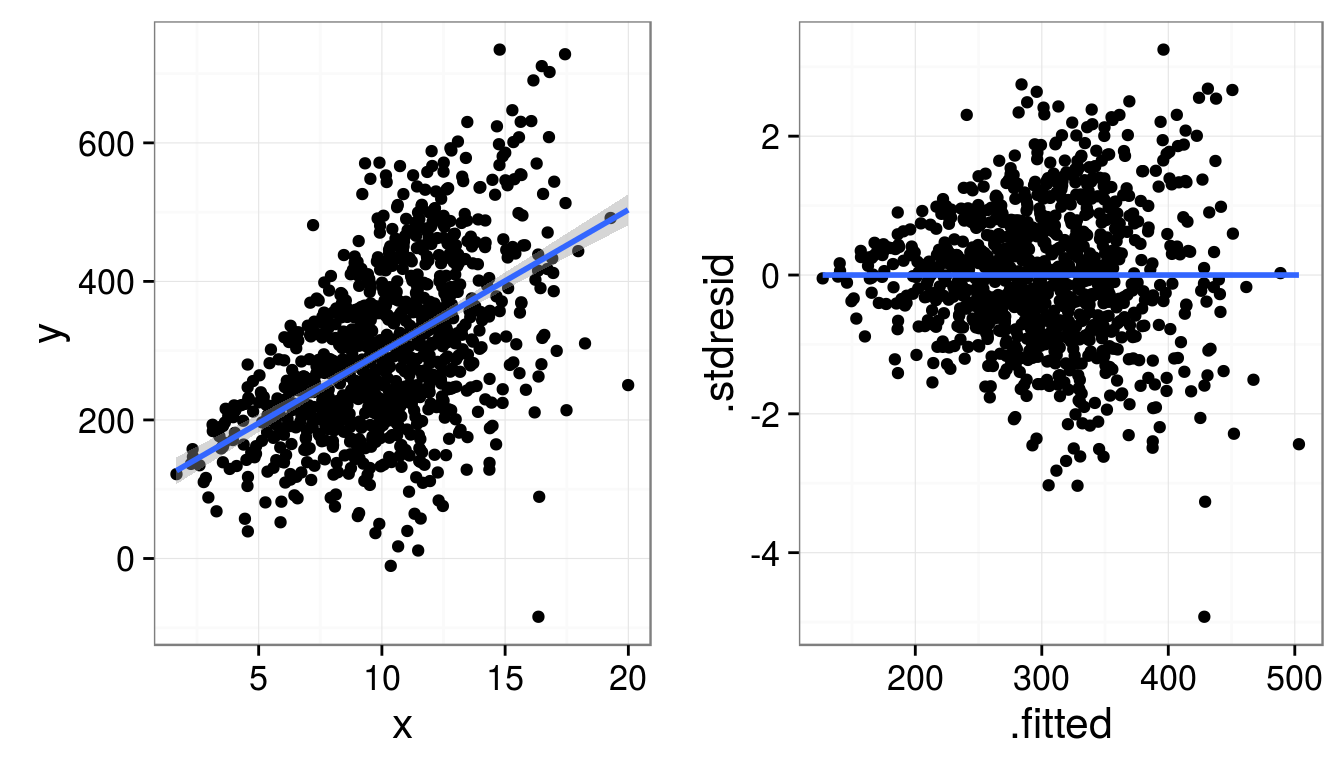
\includegraphics{11_GLM_binary2_files/figure-beamer/unnamed-chunk-14-1} \end{flushleft}

\column {0.5 \textwidth} Серая область - доверительный интервал для
логистической регрессии

Доверительные интервалы для коэффициентов:

\begin{Shaded}
\begin{Highlighting}[]
\KeywordTok{confint}\NormalTok{(liz_model) }\CommentTok{# для логитов}
\end{Highlighting}
\end{Shaded}

\begin{verbatim}
#              2.5 %  97.5 %
# (Intercept)  1.006  8.0421
# PARATIO     -0.485 -0.0665
\end{verbatim}

\begin{Shaded}
\begin{Highlighting}[]
\KeywordTok{exp}\NormalTok{(}\KeywordTok{confint}\NormalTok{(liz_model)) }\CommentTok{# для отношения шансов}
\end{Highlighting}
\end{Shaded}

\begin{verbatim}
#             2.5 %   97.5 %
# (Intercept) 2.734 3109.275
# PARATIO     0.616    0.936
\end{verbatim}

\columnsend

\end{frame}

\begin{frame}[fragile]{Задание:}

Постройте график логистической регрессии для модели \texttt{liz\_model}
без использования \texttt{geom\_smooth()}

Hint 1: Используйте функцию \texttt{predict()}, изучите значения
параметра ``type''

Hint 2: Для вызова справки напишите \texttt{predict.glm()}

Hint 3: Создайте датафрейм MyData с переменной \texttt{PARATIO},
изменяющейся от минимального до максимального значения \texttt{PARATIO}

\end{frame}

\begin{frame}[fragile]{Решение}

\columnsbegin
\column {0.5 \textwidth}

\begin{flushleft}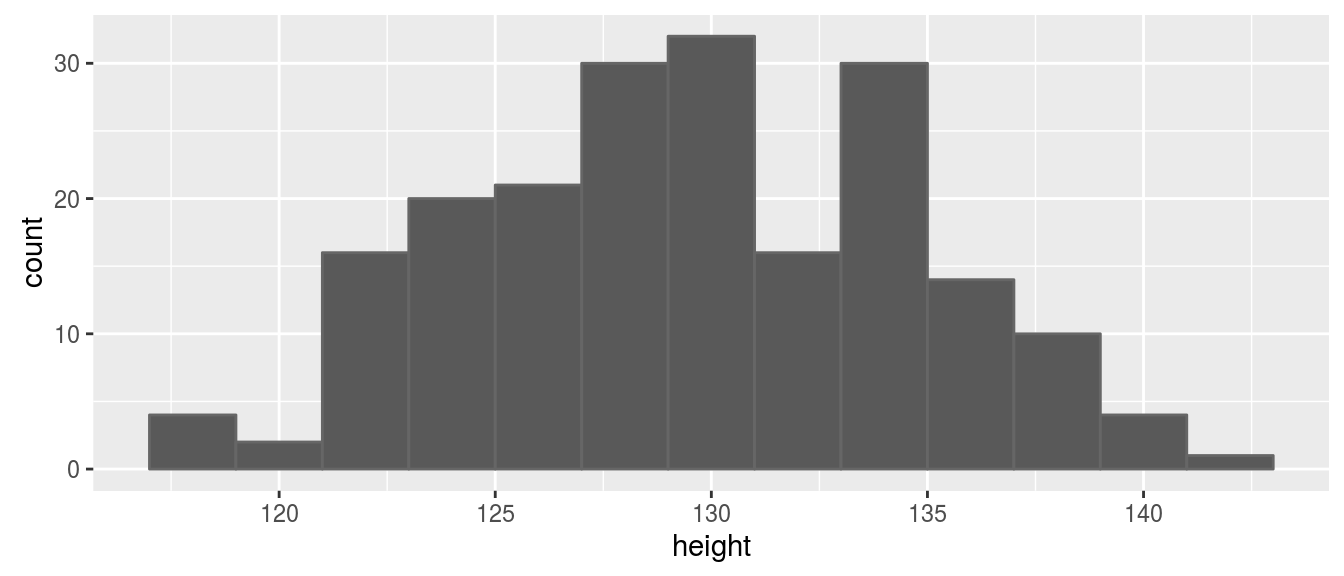
\includegraphics{11_GLM_binary2_files/figure-beamer/unnamed-chunk-16-1} \end{flushleft}

\column {0.5 \textwidth}

\begin{Shaded}
\begin{Highlighting}[]
\NormalTok{MyData <-}\StringTok{ }\KeywordTok{data.frame}\NormalTok{(}\DataTypeTok{PARATIO =}
        \KeywordTok{seq}\NormalTok{(}\KeywordTok{min}\NormalTok{(liz$PARATIO), }\KeywordTok{max}\NormalTok{(liz$PARATIO)))}

\NormalTok{MyData$Predicted <-}\StringTok{ }\KeywordTok{predict}\NormalTok{(liz_model,}
                            \DataTypeTok{newdata =} \NormalTok{MyData,}
                            \DataTypeTok{type =} \StringTok{"response"}\NormalTok{)}

\KeywordTok{ggplot}\NormalTok{(MyData, }\KeywordTok{aes}\NormalTok{(}\DataTypeTok{x =} \NormalTok{PARATIO, }\DataTypeTok{y =} \NormalTok{Predicted)) +}
\StringTok{  }\KeywordTok{geom_line}\NormalTok{(}\DataTypeTok{size=}\DecValTok{2}\NormalTok{, }\DataTypeTok{color =} \StringTok{"blue"}\NormalTok{) +}
\StringTok{  }\KeywordTok{xlab}\NormalTok{(}\StringTok{"Отношение периметра к площади"}\NormalTok{) +}
\StringTok{  }\KeywordTok{ylab} \NormalTok{(}\StringTok{"Вероятность"}\NormalTok{) +}
\StringTok{  }\KeywordTok{ggtitle}\NormalTok{(}\StringTok{"Вероятность встречи ящериц"}\NormalTok{)}
\end{Highlighting}
\end{Shaded}

\end{frame}

\begin{frame}[fragile]{Применим матричную алгебру для вычисления
предсказанных значений и доверительного интервала для линии регрессии}

\begin{Shaded}
\begin{Highlighting}[]
\CommentTok{# Создаем искуственный набор данных}
\NormalTok{MyData <-}\StringTok{ }\KeywordTok{data.frame}\NormalTok{(}\DataTypeTok{PARATIO =} \KeywordTok{seq}\NormalTok{(}\KeywordTok{min}\NormalTok{(liz$PARATIO), }\KeywordTok{max}\NormalTok{(liz$PARATIO)))}

\CommentTok{# Формируем модельную матрицу для искуственно созданных данных}
\NormalTok{X <-}\StringTok{ }\KeywordTok{model.matrix}\NormalTok{( ~}\StringTok{ }\NormalTok{PARATIO, }\DataTypeTok{data =} \NormalTok{MyData)}
\end{Highlighting}
\end{Shaded}

\end{frame}

\begin{frame}[fragile]{Извлекаем характеристики подобранной модели и
получаем предсказанные значения}

\begin{Shaded}
\begin{Highlighting}[]
\CommentTok{# Вычисляем параметры подобранной модели и ее матрицу ковариаций}
\NormalTok{betas    <-}\StringTok{ }\KeywordTok{coef}\NormalTok{(liz_model) }\CommentTok{# Векор коэффицентов}
\NormalTok{Covbetas <-}\StringTok{ }\KeywordTok{vcov}\NormalTok{(liz_model) }\CommentTok{# Ковариационная матрица}

\CommentTok{# Вычисляем предсказанные значения, перемножая модельную матрицу на вектор}
\CommentTok{# коэффициентов}
\NormalTok{MyData$eta <-}\StringTok{ }\NormalTok{X %*%}\StringTok{ }\NormalTok{betas}
\end{Highlighting}
\end{Shaded}

\end{frame}

\begin{frame}[fragile]{Получаем предсказанные значения}

\begin{Shaded}
\begin{Highlighting}[]
\CommentTok{# Переводим предсказанные значения из логитов в вероятности}
\NormalTok{MyData$Pi  <-}\StringTok{ }\KeywordTok{exp}\NormalTok{(MyData$eta) /}\StringTok{ }\NormalTok{(}\DecValTok{1} \NormalTok{+}\StringTok{ }\KeywordTok{exp}\NormalTok{(MyData$eta))}
\end{Highlighting}
\end{Shaded}

\end{frame}

\begin{frame}[fragile]{Вычисляем границы доверительного интервала}

\begin{Shaded}
\begin{Highlighting}[]
\CommentTok{# Вычисляем стандартные отшибки путем перемножения матриц}
  \NormalTok{MyData$se <-}\StringTok{ }\KeywordTok{sqrt}\NormalTok{(}\KeywordTok{diag}\NormalTok{(X %*%}\StringTok{ }\NormalTok{Covbetas %*%}\StringTok{ }\KeywordTok{t}\NormalTok{(X)))}

\CommentTok{# Вычисляем доверительные интервалы}
\NormalTok{MyData$CiUp  <-}\StringTok{ }\KeywordTok{exp}\NormalTok{(MyData$eta +}\StringTok{ }\FloatTok{1.96} \NormalTok{*MyData$se) /}
\StringTok{  }\NormalTok{(}\DecValTok{1} \NormalTok{+}\StringTok{ }\KeywordTok{exp}\NormalTok{(MyData$eta  +}\StringTok{ }\FloatTok{1.96} \NormalTok{*MyData$se))}

\NormalTok{MyData$CiLow  <-}\StringTok{ }\KeywordTok{exp}\NormalTok{(MyData$eta -}\StringTok{ }\FloatTok{1.96} \NormalTok{*MyData$se) /}
\StringTok{  }\NormalTok{(}\DecValTok{1} \NormalTok{+}\StringTok{ }\KeywordTok{exp}\NormalTok{(MyData$eta  -}\StringTok{ }\FloatTok{1.96} \NormalTok{*MyData$se))}
\end{Highlighting}
\end{Shaded}

\end{frame}

\begin{frame}[fragile]{Строим график}

\columnsbegin
\column {0.5 \textwidth}

\begin{flushleft}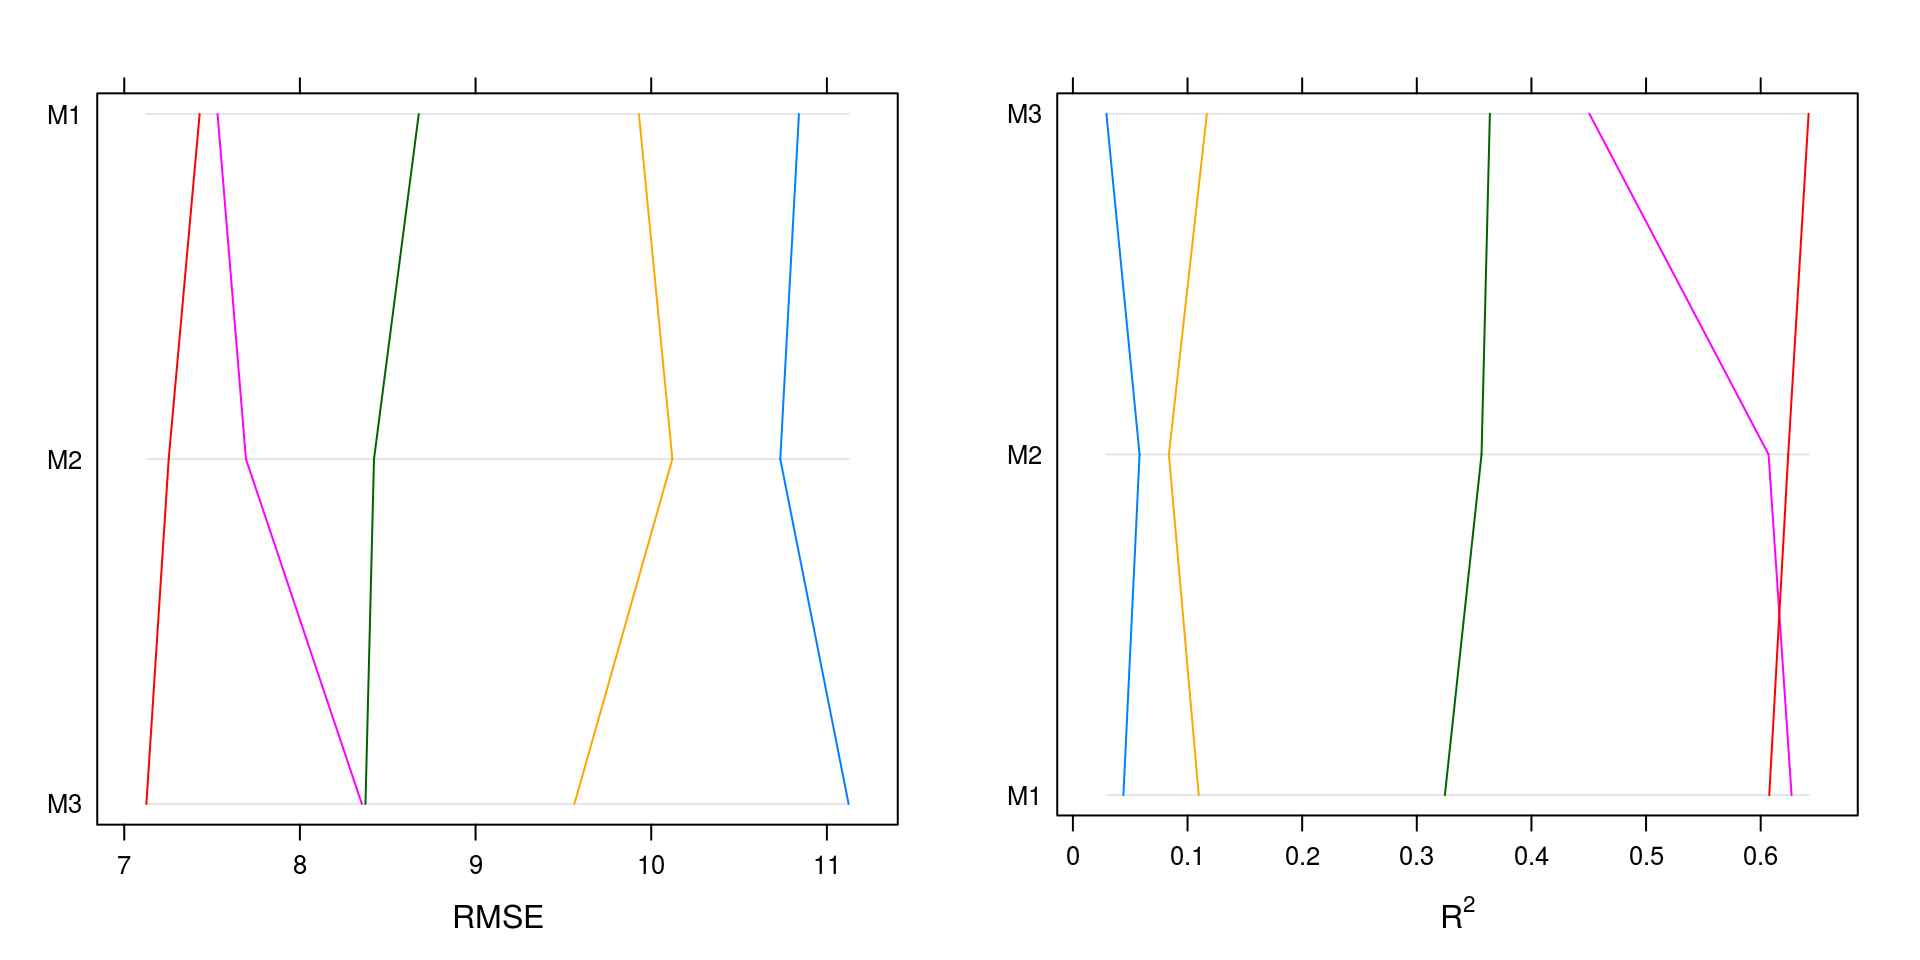
\includegraphics{11_GLM_binary2_files/figure-beamer/unnamed-chunk-22-1} \end{flushleft}

\column {0.5 \textwidth}

\begin{Shaded}
\begin{Highlighting}[]
\KeywordTok{ggplot}\NormalTok{(MyData, }\KeywordTok{aes}\NormalTok{(}\DataTypeTok{x =} \NormalTok{PARATIO, }\DataTypeTok{y =} \NormalTok{Pi)) +}
\StringTok{  }\KeywordTok{geom_line}\NormalTok{(}\KeywordTok{aes}\NormalTok{(}\DataTypeTok{x =} \NormalTok{PARATIO, }\DataTypeTok{y =} \NormalTok{CiUp),}
            \DataTypeTok{linetype =} \DecValTok{2}\NormalTok{, }\DataTypeTok{size =} \DecValTok{1}\NormalTok{) +}
\StringTok{  }\KeywordTok{geom_line}\NormalTok{(}\KeywordTok{aes}\NormalTok{(}\DataTypeTok{x =} \NormalTok{PARATIO, }\DataTypeTok{y =} \NormalTok{CiLow),}
            \DataTypeTok{linetype =} \DecValTok{2}\NormalTok{, }\DataTypeTok{size =} \DecValTok{1}\NormalTok{) +}
\StringTok{  }\KeywordTok{geom_line}\NormalTok{(}\DataTypeTok{color =} \StringTok{"blue"}\NormalTok{, }\DataTypeTok{size=}\DecValTok{2}\NormalTok{) +}
\StringTok{  }\KeywordTok{ylab}\NormalTok{(}\StringTok{"Вероятность встречи"}\NormalTok{)}
\end{Highlighting}
\end{Shaded}

\columnsend

\end{frame}

\section{Множественная логистическая регрессия}\label{--}

\end{document}
